\subsection{IPS-N Vlad}
\begin{figure}
\begin{center}
    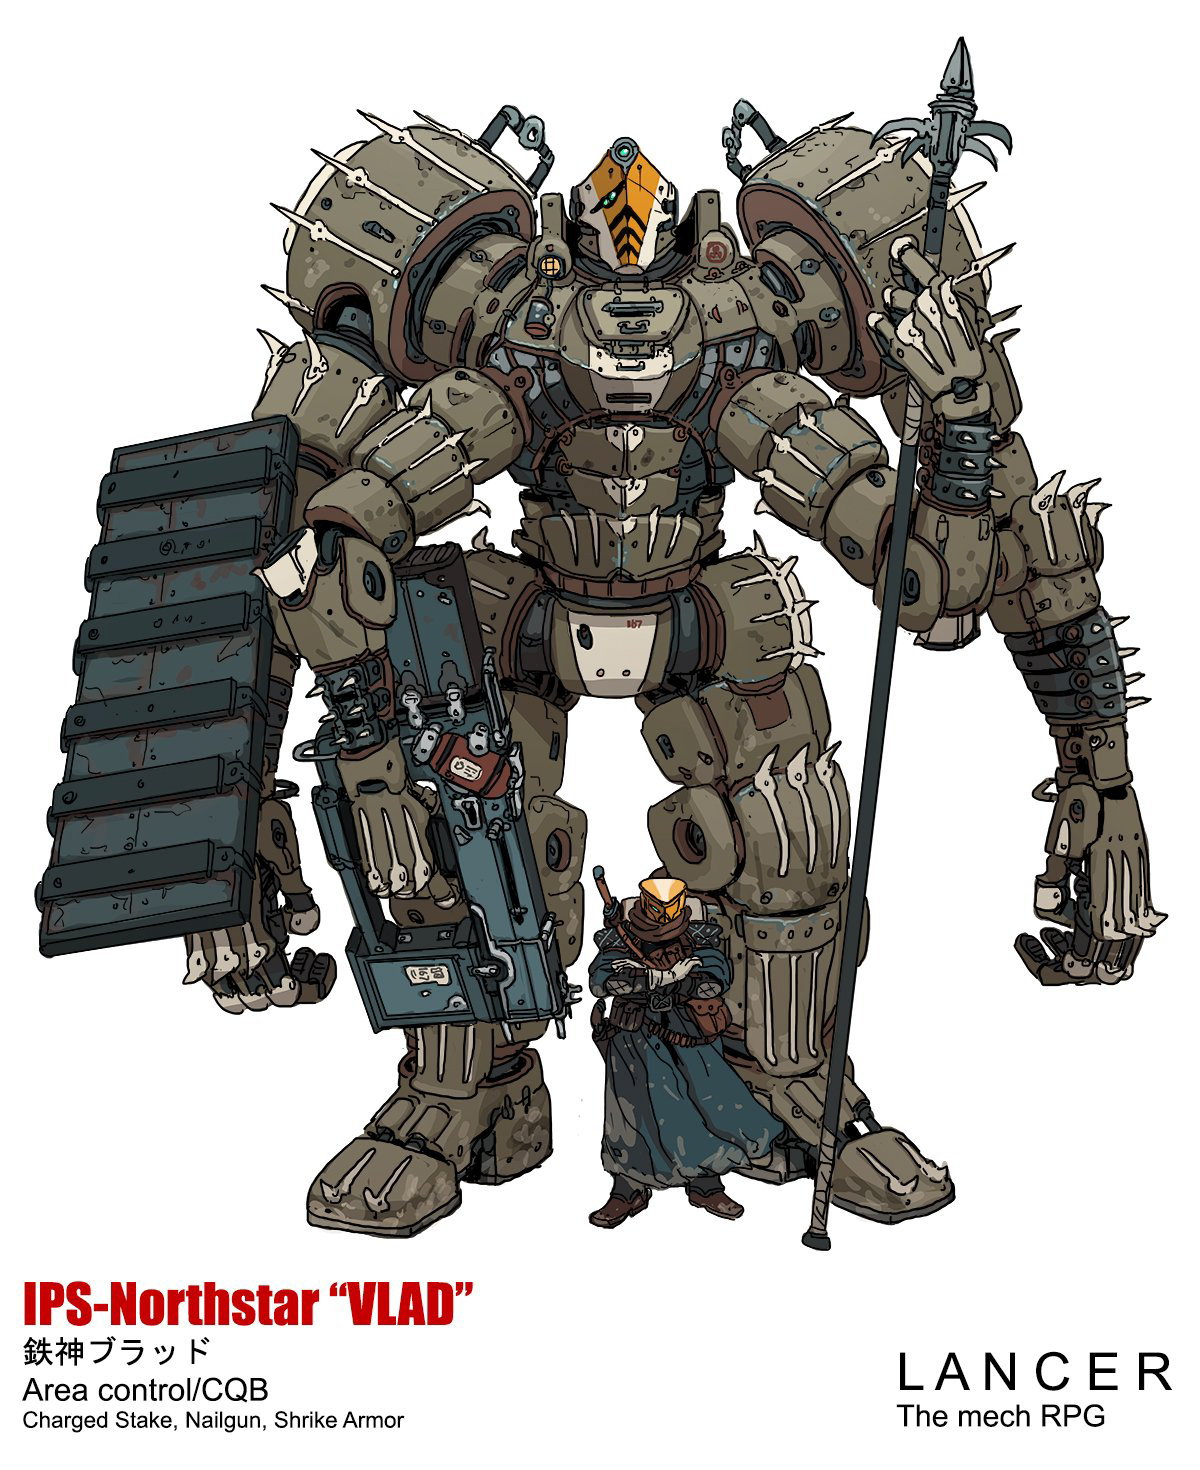
\includegraphics{Vlad}
\end{center}
\end{figure}
\begin{mech}{IPS-N}{Vlad}

\fluff{The IPS-N VLAD is a variant of the IPS-N NELSON, built to handle hardened targets that would present strategic difficulty for the NELSON platform. The VLAD features a suite of myth-inspired weaponry and heavy armor and is meant to take a frontline role, absorbing fire from dangerous targets in order to protect its allies while lining up the perfect shot.}

\begin{license}
\item Snare Trap, Impact Lance
\item VLAD FRAME, Nail Gun, Caltrop Launcher
\item Combat Drill, Charged Stake
\end{license}

\frameBox
[hp = 10,
evasion = 8,
speed = 4,
heat cap = 4,
sensors = 5,
armor = 2,
e-defense = 8,
size = 1,
repair cap = 4,
tech attack = +0,
traits = {\textbf{Dismemberment:} When the Vlad successfully immobilizes a target, that target is also Shredded for the same duration

\textbf{Shrike Armor:} When the Vlad is attacked by any actor within range 3, the attacker takes 1 AP kinetic damage before they attack
},
sp = 5,
mount one = flex mount,
mount two = main mount,
mount three = heavy mount,
core system name = Shrike Armor,
core system text = {A nod to the pre-Fall namesake of the VLAD, Shrike armor plating bristles with shaped spikes, hardened with chromium/tungsten alloy tips. Strategic studding places Shrike tips in high-likelihood kinetic encounter areas: gauntlet covers, manipulator joint covers, shoulder plating, and so on. Primarily a defensive modification, Shrike armor is uncommon among Coreside pilots, and seen as a mark of underdeveloped -- if terrifying - tactics.},
core active name = Tormentor spines,
core active text = {Protocol

Until the end of the current challenge, you gain resistance to all damage from within range 3, and your damage from this armor's passive increases to 3 AP kinetic damage.}]


Snare Trap
The IPS-N WEBJAW Explosively-Accelerated Filament system is a deployable all-theater perimeter defense system designed to arrest hostile movement in pre-determined kill-corridors. Deployable by hand or launch tube, the WEBJAW EAF system consists of a cluster of filament anchors scattered across an area. When triggered remotely or by a series of programmable physical, electronic, or chemical triggers, the anchors target and fire at the triggering foe, embedding hard-tip barbs deep inside both hard and soft targets. The barbs, anchored to their bases by arachnosilk-analog filament, immobilize and entangle the target.

1 SP
Mine, Limited 1
This trap triggers when any actor passes directly over it. The target must pass a hull check or take 2d6 AP kinetic damage and become immobilized. Once triggered, the trap becomes an object with 10 HP and 5 evasion, and immobilizes its target as long as it is not destroyed.

Impact Lance
The Impact Lance is a milspec variant of a common mining tool: the single-use, proximal-distance chemical survey laser. IPS-N's military variant mounts a series of Impact Lances on a brachial or thoracic carriages, leaving a chassis' manipulators free to field other weapons and systems; the Lance can be wired directly into a chassis' core, or charged with single-use chemical batteries.

The lances fire for a microsecond, burning through their stored charge in a milisolar burst of light that stabs out in a tight, pulsed beam capable of searing through multiple meters of hardened bulkhead.

Main Melee
Threat 2
1d6 energy damage
This weapon attacks in a line drawn between its target and your mech, attacking all other actors in between, but deals +1 heat to your mech for each target hit past the first

IPS-N ``Impaler'' Nailgun
The milspec Nailgun utilizes non-combustible, sabot-jacketed two-stage macroflechettes to pierce even the most substantial of armor. First catapulted from its launcher, the macroflechette's sabot disengages on approach to its target, triggering a second stage where internal propulsion drives the macroflechette forward with incredible velocity. Against soft targets, over-penetration is certain: IPS-N advises pilots employ this weapon platform only when the area behind the target is clear of allies and/or noncombatants.

Main CQB
1 heat (self)
Range 8, Threat 3
1d6 kinetic damage
On a Critical Hit, the target of this attack must pass a hull check or be immobilized until the end of its next turn

Caltrop Launcher
A wicked anti-organic, anti-vehicle, proximity denial system, chassis-mounted caltrops are fired in great clouds of shimmering metal (or deployed in long swathes) to blanket an area.

IPS-N's HX-CAL caltrop system adds small, shaped explosives to the mix of hardened pyramids.

1 SP, Unique
Quick Action
When this system is activated, your mech targets a free space within range 5 and blankets a blast 1 area centered on that space with explosive caltrops. That area becomes difficult terrain, and mechs moving across the space (voluntarily or otherwise) take 1 AP explosive damage for each space they move.

Combat Drill
The IPS-N combat drill is a brutal close combat weapon, powered by a massive catalyst pack mounted externally on a mech core. The drill is tipped with micro-plasmatic projectors designed to pre-treat the target to ensure bit purchase and facilitate drill penetration.

Superheavy Melee
Overcharged, AP
Threat 1
3d6 kinetic + 1d6 energy

Charged Stake
Built from gear meant originally for blast mining, this enormous, improvised system is loaded and cocked prior to embark into a specially primed chamber. It is designed to penetrate and immobilize hardened targets, then send powerful, vaporizing charges into its vulnerable internal systems.

2 SP
Full Action
This brutal system can be used against any adjacent target. That target must pass a hull check with 1 difficulty or take 2d6 energy damage damage and become immobilized and impaled. At the end of each of its turns, the target can repeat this check to end the effect on itself, otherwise it takes 3 AP energy damage and remains immobilized until it makes the check successfully. Only one target can be immobilized by this system at once, but it can be picked up as a quick action.


\end{mech}
